\documentclass{ximera}
\graphicspath{     %% setup a global graphics path
{./}               %% look in the same-level directory
{./pictures/}      %% look in graphics
{../pictures/}     %% look up one directory, then in graphics
%{../../pictures/} %% look up two directories, then in graphics
}

\author{Zack Reed}
\title{Matrix Multiplication}

\begin{document}

\begin{abstract}

\end{abstract}
\maketitle

\section*{Properties of Matrix Multiplication}

    One might expect that, with how much more nuanced matrix multiplication and matrix-vector multiplication are compared to scalar multiplication, that there would be some extra rules and constraints.

    We'll explore these below.

    \begin{example}\name{Allowed mulitplications}

        Whereas we can multiply any scalar by another scalar (unelss we divide by zero), the same is not true for matrices, and also for matrix-vector multiplication.

        The key consideration is that matrices transform vectors in $\R^n$ to vectors in $\R^m$, and so we need to make sure that the matrices are defined to take in $n$-dimensional vectors and output $m$-dimensional vectors.

        Let's use some mapping diagrams to illustrate this for the $3\times 2$ matrix \(M=\begin{bmatrix} 1 & 2 \\ 2&-1 \\ 1 & 1\end{bmatrix}\)

        If $\vec{v}= \begin{bmatrix} 2 \\ 3 \end{bmatrix}$, then $M\vec{v}$ is calculated by $M\vec{v}=2 \begin{bmatrix} 1 \\ 2 \\ 1 \end{bmatrix}+3 \begin{bmatrix} 2 \\ -1 \\ 1 \end{bmatrix}=\begin{bmatrix} 2+6 \\ 4-3 \\ 2+3 \end{bmatrix}=\begin{bmatrix} 8 \\ 1 \\ 5 \end{bmatrix}$.

        Since the columns of $M$ are $3$-dimensional, the result is a $3$-dimensional vector (one for each vector in the linear combination). Since the rows of $M$ are $2$-dimensional, the input vector must be $2$-dimensional (one for each scalar in the linear combination).

        By contrast, if $\vec{v}= \begin{bmatrix} 2 \\ 3 \\ 4 \end{bmatrix}$, then $M\vec{v}$ does not make sense because there isn't a third column of $M$ to multiply by the third entry of $\vec{v}$.

        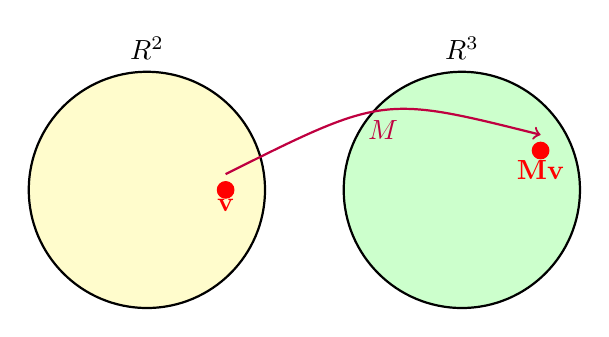
\begin{tikzpicture}

            % Draw sets X, X'
            \draw[fill=yellow!20!white, draw=black, thick] (-4,0) ellipse (1.5cm);
            \draw[fill=green!20!white, draw=black, thick] (0,0) ellipse (1.5cm);
        
            % Labels for sets X, X'
            \node at (-4,1.8) {\(\mathbb{R}^2\)};
            \node at (0,1.8) {\(\mathbb{R}^3\)};
        
            % Elements inside sets
            \filldraw[red] (-3,0) circle (3pt) node[below] {\textbf{v}};
            \filldraw[red] (1,.5) circle (3pt) node[below] {\textbf{Mv}};
        
            % Arrows for the transformation S
            \draw[->, thick, purple] (-3,0.2) .. controls (-1,1.2) .. (1,.7) node[midway, below] {\(M\)};
            
        \end{tikzpicture}

        Detemrine which of the following multiplications make sense, and why.

        $M=\begin{bmatrix} 1 & 2 \\ 2&-1 \\ 1 & 1\end{bmatrix}$, $N=\begin{bmatrix} 1 & 2 & 3 \\ 2&-1 & 0 \\ 1 & 1 & 1\end{bmatrix}$, $P=\begin{bmatrix} 1 & 2 \\ 2&-1 \\ 1 & 1 \\ 0 & 0\end{bmatrix}$

        $v=\begin{bmatrix} 2 \\ 3 \end{bmatrix}$,
        $w=\begin{bmatrix} 2 \\ 3 \\ 4 \end{bmatrix}$, $u=\begin{bmatrix} 2 \\ 3 \\ 4 \\ 5 \end{bmatrix}$

        Select all products that are allowed, make sure that the dimensional description is also correct.

        \begin{selectAll}

            \choice[correct]{$Mv$ is a $3$-dimensional vector}
            \choice{$Mv$ is a $2$-dimensional vector}
            \choice{$Mw$ is a $3$-dimensional vector}
            \choice{$Mw$ is a $2$-dimensional vector}
            \choice{$Mu$ is a $4$-dimensional vector}
            \choice{$Mu$ is a $3$-dimensional vector}
            \choice{$Nv$ is a $3$-dimensional vector}
            \choice{$Nv$ is a $2$-dimensional vector}
            \choice[correct]{$Nw$ is a $3$-dimensional vector}
            \choice{$Nw$ is a $2$-dimensional vector}
            \choice{$Nu$ is a $4$-dimensional vector}
            \choice{$Nu$ is a $3$-dimensional vector}
            \choice[correct]{$Pv$ is a $4$-dimensional vector}
            \choice{$Pv$ is a $3$-dimensional vector}
            \choice{$Pw$ is a $4$-dimensional vector}
            \choice{$Pw$ is a $3$-dimensional vector}
            \choice{$Pu$ is a $4$-dimensional vector}
            \choice{$Pu$ is a $3$-dimensional vector}
        \end{selectAll}

        \begin{solution}

            The matrix $M=\begin{bmatrix} 1 & 2 \\ 2&-1 \\ 1 & 1\end{bmatrix}$ is $3\times 2$, so it can only multiply $2$-dimensional vectors. $Mv$ produces a $3$-dimensional vector from its $3$ rows. 

            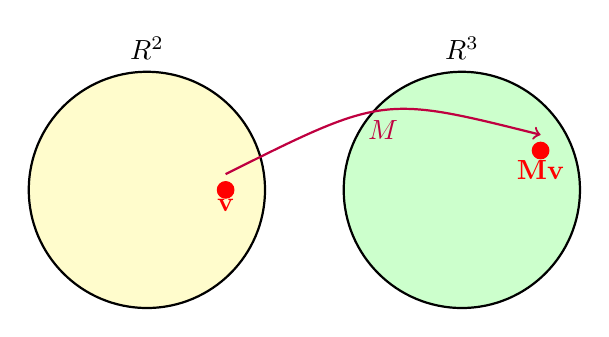
\begin{tikzpicture}

                % Draw sets X, X'
                \draw[fill=yellow!20!white, draw=black, thick] (-4,0) ellipse (1.5cm);
                \draw[fill=green!20!white, draw=black, thick] (0,0) ellipse (1.5cm);
            
                % Labels for sets X, X'
                \node at (-4,1.8) {\(\mathbb{R}^2\)};
                \node at (0,1.8) {\(\mathbb{R}^3\)};
            
                % Elements inside sets
                \filldraw[red] (-3,0) circle (3pt) node[below] {\textbf{v}};
                \filldraw[red] (1,.5) circle (3pt) node[below] {\textbf{Mv}};
            
                % Arrows for the transformation S
                \draw[->, thick, purple] (-3,0.2) .. controls (-1,1.2) .. (1,.7) node[midway, below] {\(M\)};
                
            \end{tikzpicture}

            The matrix $N=\begin{bmatrix} 1 & 2 & 3 \\ 2&-1 & 0 \\ 1 & 1 & 1\end{bmatrix}$ is a $3\times 3$ matrix,
            so it can only multiply $3$-dimensional vectors. $Nw$ produces a $3$-dimensional vector from its $3$ rows.

            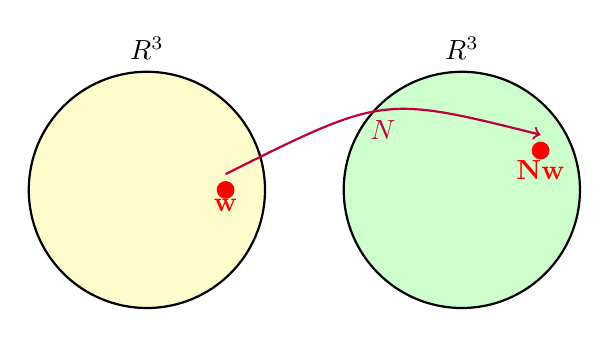
\begin{tikzpicture}

                % Draw sets X, X'
                \draw[fill=yellow!20!white, draw=black, thick] (-4,0) ellipse (1.5cm);
                \draw[fill=green!20!white, draw=black, thick] (0,0) ellipse (1.5cm);
            
                % Labels for sets X, X'
                \node at (-4,1.8) {\(\mathbb{R}^3\)};
                \node at (0,1.8) {\(\mathbb{R}^3\)};
            
                % Elements inside sets
                \filldraw[red] (-3,0) circle (3pt) node[below] {\textbf{w}};
                \filldraw[red] (1,.5) circle (3pt) node[below] {\textbf{Nw}};
            
                % Arrows for the transformation N
                \draw[->, thick, purple] (-3,0.2) .. controls (-1,1.2) .. (1,.7) node[midway, below] {\(N\)};
            
            \end{tikzpicture}

            The matrix $P=\begin{bmatrix} 1 & 2 \\ 2&-1 \\ 1 & 1 \\ 0 & 0\end{bmatrix}$ is $4\times 2$, so it can only multiply $2$-dimensional vectors. $Pv$ produces a $4$-dimensional vector from its $4$ rows.

            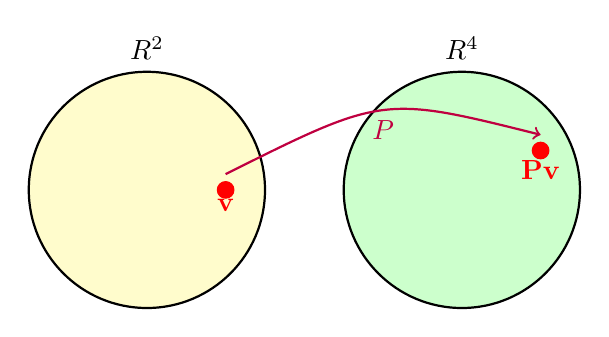
\begin{tikzpicture}

                % Draw sets X, X'
                \draw[fill=yellow!20!white, draw=black, thick] (-4,0) ellipse (1.5cm);
                \draw[fill=green!20!white, draw=black, thick] (0,0) ellipse (1.5cm);
            
                % Labels for sets X, X'
                \node at (-4,1.8) {\(\mathbb{R}^2\)};
                \node at (0,1.8) {\(\mathbb{R}^4\)};
            
                % Elements inside sets
                \filldraw[red] (-3,0) circle (3pt) node[below] {\textbf{v}};
                \filldraw[red] (1,.5) circle (3pt) node[below] {\textbf{Pv}};
            
                % Arrows for the transformation P
                \draw[->, thick, purple] (-3,0.2) .. controls (-1,1.2) .. (1,.7) node[midway, below] {\(P\)};
            
            \end{tikzpicture}

        \end{solution}

        With matrix multiplication, you have to smimilalry consider the dimensions of the vectors after each successive multiplication. You simply need to apply the same reasoning as matrix-vector mulitplication, but keep in mind the dimensions of the output vectors from the first product. If we take the matrices $M$ and $N$ from the previous example, $MN$ would not be allowed because the output of $N$ is $3$-dimensional, and the input of $M$ is $2$-dimensional, so the product would not be defined. 

        $NM$, however, would be allowed because the output of $M$ is $3$-dimensional, and the input of $N$ is $3$-dimensional, so the product would be defined.

        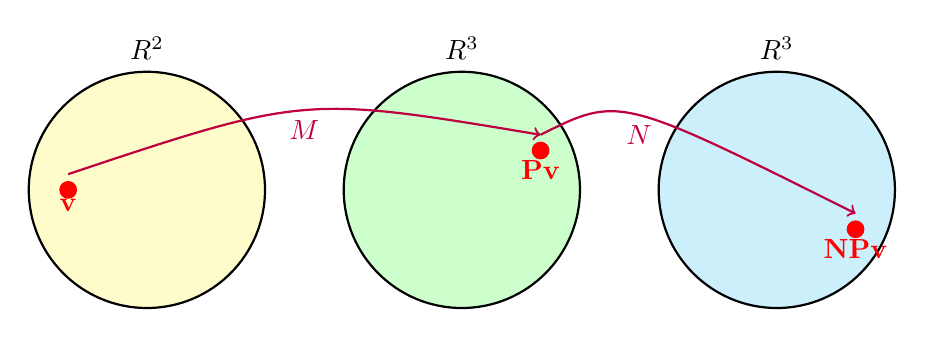
\begin{tikzpicture}

            % Draw sets X, X', and X''
            \draw[fill=yellow!20!white, draw=black, thick] (-4,0) ellipse (1.5cm);  % First ellipse (R^2)
            \draw[fill=green!20!white, draw=black, thick] (0,0) ellipse (1.5cm);    % Second ellipse (R^4)
            \draw[fill=cyan!20!white, draw=black, thick] (4,0) ellipse (1.5cm);     % Third ellipse (R^3)
        
            % Labels for sets X, X', X''
            \node at (-4,1.8) {\(\mathbb{R}^2\)};
            \node at (0,1.8) {\(\mathbb{R}^3\)};
            \node at (4,1.8) {\(\mathbb{R}^3\)};
        
            % Elements inside sets
            \filldraw[red] (-5,0) circle (3pt) node[below] {\textbf{v}};  % Vector in R^2
            \filldraw[red] (1,.5) circle (3pt) node[below] {\textbf{Pv}}; % Vector in R^4
            \filldraw[red] (5,-.5) circle (3pt) node[below] {\textbf{NPv}}; % Vector in R^3
        
            % Arrows for the transformations P and N
            \draw[->, thick, purple] (-5,0.2) .. controls (-2,1.2) .. (1,.7) node[midway, below] {\(M\)};
            \draw[->, thick, purple] (1,.7) .. controls (2,1.2) .. (5,-.3) node[midway, below] {\(N\)};
        
        \end{tikzpicture}

        Now determine which of the following matrix products is allowed, and why, using the matrices %make a 2x3, 3x4, 2x2, 3x3 matrices
        $M=\begin{bmatrix} 1 & 2 & 1\\ 2&-1 &0\end{bmatrix}$, $N=\begin{bmatrix} 1 & 2 & 3 \\ 2&-1 & 0 \\ 1 & 1 & 1 \\ 0 & 0 & 0\end{bmatrix}$, $P=\begin{bmatrix} 1 & 2 \\ 2&-1 \end{bmatrix}$, $Q=\begin{bmatrix} 1 & 2 & 3 \\ 2&-1 & 0 \\ 1 & 1 & 1\end{bmatrix}$.


        \begin{selectAll}

            \choice{$MN$}
            \choice[correct]{$MN^T$}
            \choice{$NM$}
            \choice{$NM^T$}
            \choice{$MP$}
            \choice[correct]{$M^TP$}
            \choice{$PQ$}
            \choice{$QP$}
            \choice{$PQ^T$}
            \choice[correct]{$NQ$}
            \choice{$N^TQ$}
            \choice[correct]{$PM$}

        \end{selectAll}

        \begin{solution}
        
            $N^T$ is a $3\times 4$ matrix, so it outputs a $3$-dimensional vector. $M$ is a $2\times 3$ matrix, so it takes in a $3$-dimensional vector and thus the product $MN^T$ is allowed.

            $P$ is a $2\times 2$ matrix, so it outputs a $2$-dimensional vector. $M^T$ is a $3\times 2$ matrix, so it takes in a $2$-dimensional vector and thus the product $M^TP$ is allowed.

            $Q$ is a $3\times 3$ matrix, so it outputs a $3$-dimensional vector. $N$ is a $4\times 3$ matrix, so it takes in a $3$-dimensional vector and thus the product $NQ$ is allowed.

            $M$ is a $2\times 3$ matrix, so it outputs a $2$-dimensional vector. $P$ is a $2\times 2$ matrix, so it takes in a $2$-dimensional vector and thus the product $PM$ is allowed.

        \end{solution}

    \end{example}

    \begin{example}\name{Commutativity}

        Scalar multiplication is commutative, meaning you can swap the order of any numbers in the product and still get the same result.

        For instance, $3\cdot 4\cdot 5\cdot 2=2\cdot 5\cdot 4\cdot 3=4\cdot 3\cdot 5\cdot 2=120$.

        Let's check whether we can do the same for matrix multiplication. In our past example, we got the composite matrix $M=FRS$, a stretch by $2$, a $60^\circ$ rotation, and a reflection about the $y$-axis.

        If matrix multiplication is commutative, then the matrices $FSR$ and $RFS$ should give us the same result as $M$, since it wouldn't matter what order we multiplied the matrices in.

        Do this in MATLAB and match the results of each product.

        \begin{hint}

            You can use the same code as before, but just change the order of the matrices in the product. Match each figure to the matrices that produced them.

        \end{hint}

        % Include the FSR image
        \begin{figure}[ht!]
            \centering
            \includegraphics[width=\textwidth]{fsr.png}
            \caption{(a)}
        \end{figure}
        
        \begin{selectAll}

            \choice[correct]{$FSR$}
            \choice{$RSF$}
            \choice[correct]{$SFR$}
            \choice{$SRF$}

        \end{selectAll}

        % Include the SRF image
        \begin{figure}[ht!]
            \centering
            \includegraphics[width=\textwidth]{srf.png}
            \caption{(c)}
        \end{figure}

        \begin{selectAll}

            \choice{$FSR$}
            \choice{$RSF$}
            \choice{$SFR$}
            \choice[correct]{$SRF$}           

        \end{selectAll}

        % Include the RSF image
        \begin{figure}[ht!]
            \centering
            \includegraphics[width=\textwidth]{rsf.png}
            \caption{(d)}
        \end{figure}

        \begin{selectAll}

            \choice{$FSR$}
            \choice[correct]{$RSF$}
            \choice{$SFR$}
            \choice{$SRF$}

        \end{selectAll}

    As we can see, while there is some overlap, different orders of matrix multiplication produced different transformations of the inptu vectors in $\R^2$. We have to conclude that the ordering matters for matrix multiplication, and so \emph{matrix multiplication is not commutative}.

    \end{example}

    \begin{example}\name{Associativity}

        Associativity regards the order in which each pair of operations is carried out. For instance, $(3\cdot 4)\cdot 5=12\cdot 5=60$, and $3\cdot (4\cdot 5)=3\cdot 20=60$, so even though we carried out each multiplication in a different order, we still got the same result.

        Is this also true for matrices? Let's check.

        Use the following code, which computes each pair of matrices before the for loop, and then apply the pairs in different orders to check for associativity.

        First, compute $F(RS)$.

        \vspace{1cm}


\texttt{load +linalg/face\textunderscore points.mat}

\texttt{R = [cosd(60) -sind(60); sind(60) cosd(60)]}

\texttt{S = [1 0; 0 2]}

\texttt{F = [-1 0; 0 1]}

\texttt{RS = }$\answer[given,format=string]{R}*\answer[format=string]{S}$

\texttt{FR = }$\answer[given,format=string]{F}*\answer[format=string]{R}$

\texttt{for i=1:length(face\textunderscore points)}

$\qquad $\texttt{face\textunderscore points(i,:) = }$\answer[given,format=string]{RS}$\texttt{*face\textunderscore points(i,:)';}

$\qquad $\texttt{face\textunderscore points(i,:) = }$\answer[format=string]{F}$\texttt{*face\textunderscore points(i,:)';}

\texttt{end}

\texttt{linalg.plot\textunderscore img\textunderscore points(face\textunderscore points)}

\vspace{1cm}

        Then, compute $(FR)S$.

        \vspace{1cm}

\texttt{for i=1:length(face\textunderscore points)}

$\qquad $\texttt{face\textunderscore points(i,:) = }$\answer[given,format=string]{S}$\texttt{*face\textunderscore points(i,:)';}

$\qquad $\texttt{face\textunderscore points(i,:) = }$\answer[format=string]{FR}$\texttt{*face\textunderscore points(i,:)';}

$\texttt{end}$

\texttt{linalg.plot\textunderscore img\textunderscore points(face\textunderscore points)}

\vspace{1cm}

These should all give you the same smiley face that we originally stretched, rotated, and reflected.

So, matrix multiplicaiton \emph{is associative}.

    \end{example}

\section*{Review Video}

\begin{remark}

    As we continue to learn more properties of matrices, and which matrices are useful for solving various problems, remember that most (if not all) of the powerful things that we can do with matrices boil down to the understanding of matrices as linear transformations.

\end{remark}

There's a lot to review, and we'll be doing much more with linear transformations moving forward. Here's a helpful summary from Grant Sanderson:

\youtube{kYB8IZa5AuE?si=pfb2PjvAwHiPSl5X}

\end{document}